% Importado desde: 2026-03-28_Nielsen_Ninomiya_y_Doblamento_Fermionico.tex
\chapter{Derivacion Pedagogica: --- Nielsen--Ninomiya, doblamiento fermionico y el limite Dirac en red}
\label{ch:nielsen-ninomiya-doblamento}






% verified-by: validators/nielsen_ninomiya.py::test_even_nodes_satisfiable
% verified-by: validators/nielsen_ninomiya.py::test_odd_nodes_unsatisfiable
% verified-by: validators/nielsen_ninomiya.py::test_no_uniform_chirality
% verified-by: validators/nielsen_ninomiya.py::test_balanced_count
% verified-by: validators/wilson_subsector.py::test_massless_at_zero
% verified-by: validators/wilson_subsector.py::test_doubler_mass_at_pi
% verified-by: validators/wilson_subsector.py::test_linearization_is_dirac
% verified-by: validators/wilson_subsector.py::test_squared_at_corners

\section{Objetivo}

En los documentos anteriores ya aparecieron tres ideas importantes:

\begin{enumerate}[leftmargin=*]
  \item una red discreta puede producir un Hamiltoniano efectivo tipo Dirac;
  \item esa emergencia aparece al linealizar alrededor de nodos;
  \item la estructura interna por celda unitaria actua como un pseudospin efectivo.
\end{enumerate}

Pero falta el obstaculo central del programa: \textbf{una red ingenua no produce un solo fermion quiral o un solo cono de Dirac aislado de la forma que uno quisiera}. En cuanto imponemos localidad, hermiticidad y periodicidad de la zona de Brillouin, aparecen copias extra. A este fenomeno se le llama \textbf{doblamiento fermionico}, y su formulacion rigurosa esta encapsulada en el teorema de Nielsen--Ninomiya.

La meta de este capitulo es explicar ese resultado paso a paso, empezando por la intuicion mas simple en una dimension y avanzando hacia la formulacion general relevante para el proyecto.

\section{La intuicion basica: por que una red trae periodicidad}

En una teoria continua, el momento \(p\) puede recorrer toda la recta. En una red, en cambio, el momento de Bloch \(k\) vive en una region compacta: la \textbf{zona de Brillouin}. En una dimension:
\begin{equation}
k \in \left[-\frac{\pi}{a},\frac{\pi}{a}\right],
\end{equation}
donde \(a\) es el espaciamiento de red.

Eso ya cambia toda la historia. Una derivada espacial continua
\begin{equation}
\partial_x \longrightarrow \ii p
\end{equation}
se reemplaza, en una discretizacion local simple, por una funcion periodica de \(k\), tipicamente
\begin{equation}
\partial_x \;\leadsto\; \frac{1}{2a}\bigl(\psi_{n+1}-\psi_{n-1}\bigr)
\quad\Longrightarrow\quad
\ii p \;\leadsto\; \frac{\ii}{a}\sin(ka).
\end{equation}

La linealidad \(p\) de la teoria continua se vuelve entonces una funcion periodica \(\sin(ka)\). Esa periodicidad es la semilla del doblamiento: si una funcion periodica vale cero en un punto y cambia de signo, es muy dificil impedir que vuelva a anularse en otros lugares de la zona de Brillouin.

\begin{figure}[ht]
\centering
\begin{tikzpicture}[>=Latex,scale=1.05]
  \draw[->] (-4,0) -- (4,0) node[right] {\(k\)};
  \draw[->] (0,-1.4) -- (0,1.5) node[above] {\(\sin(ka)\)};
  \draw[domain=-3.1416:3.1416,smooth,samples=200,very thick,blue!70!black]
    plot (\x, {sin(\x r)});
  \draw[dashed] (-3.1416,-1.2) -- (-3.1416,1.2);
  \draw[dashed] (3.1416,-1.2) -- (3.1416,1.2);
  \fill[red!75!black] (0,0) circle (2.3pt);
  \fill[red!75!black] (-3.1416,0) circle (2.3pt);
  \fill[red!75!black] (3.1416,0) circle (2.3pt);
  \node[below] at (-3.1416,0) {\(\,-\pi/a\)};
  \node[below] at (0,0) {\(0\)};
  \node[below] at (3.1416,0) {\(\pi/a\)};
  \node[above right] at (1.1,0.9) {\small derivada discreta};
\end{tikzpicture}
\caption{Una discretizacion local simple convierte el momento lineal en una funcion periodica. Los ceros en la zona de Brillouin son inevitables y preparan el doblamiento fermionico.}
\label{c26:fig:sin-periodic}
\end{figure}

\section{Primer ejemplo: fermion de Dirac ingenuo en una dimension}

\subsection{Partimos del continuo}

Tomemos el Hamiltoniano de Dirac mas simple en una dimension espacial:
\begin{equation}
H = \alpha\, p + \beta\, m,
\label{c26:eq:dirac-cont}
\end{equation}
donde \(\alpha\) y \(\beta\) son matrices \(2\times 2\) que satisfacen
\begin{equation}
\alpha^2 = \beta^2 = \mathbb{I},
\qquad
\{\alpha,\beta\}=0.
\end{equation}

Una eleccion natural es
\begin{equation}
\alpha = \sigma_x,
\qquad
\beta = \sigma_z.
\end{equation}

Entonces el espectro es
\begin{equation}
E(p) = \pm \sqrt{p^2 + m^2}.
\end{equation}

Cuando \(m=0\), hay un unico cruce lineal en \(p=0\).

\subsection{Ahora discretizamos el espacio}

Si el espacio es una red unidimensional con espaciado \(a\), la derivada central reemplaza al momento por
\begin{equation}
p \longrightarrow \frac{1}{a}\sin(ka).
\end{equation}

El Hamiltoniano de Bloch ingenuo queda
\begin{equation}
H(k) = \frac{1}{a}\sin(ka)\,\sigma_x + m\,\sigma_z.
\label{c26:eq:naive-1d}
\end{equation}

Su espectro es
\begin{equation}
E(k)=\pm \sqrt{\frac{1}{a^2}\sin^2(ka)+m^2}.
\label{c26:eq:disp-naive-1d}
\end{equation}

Ya vemos el problema:

\begin{enumerate}[leftmargin=*]
  \item si \(m\neq 0\), el sistema tiene gap;
  \item si \(m=0\), los cruces aparecen cuando \(\sin(ka)=0\);
  \item en la zona de Brillouin eso ocurre en \(k=0\) y en \(k=\pi/a\) (equivalentemente en el borde).
\end{enumerate}

En otras palabras: \textbf{queriamos un fermion sin masa; la red nos dio dos}.

\begin{figure}[ht]
\centering
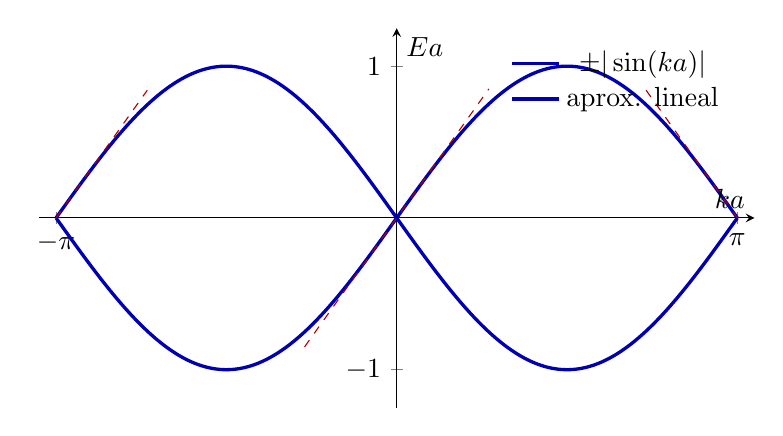
\begin{tikzpicture}
\begin{axis}[
  width=0.88\textwidth,
  height=6.4cm,
  domain=-3.1416:3.1416,
  samples=300,
  xmin=-3.3,xmax=3.3,
  ymin=-1.25,ymax=1.25,
  axis lines=middle,
  xlabel={\(ka\)},
  ylabel={\(Ea\)},
  xtick={-3.1416,0,3.1416},
  xticklabels={\(-\pi\),\(0\),\(\pi\)},
  ytick={-1,0,1},
  legend style={draw=none,fill=none,at={(0.97,0.97)},anchor=north east}
]
\addplot[very thick,blue!70!black] {abs(sin(deg(x)))};
\addplot[very thick,blue!70!black] {-abs(sin(deg(x)))};
\addplot[dashed,red!70!black,domain=-0.85:0.85] {x};
\addplot[dashed,red!70!black,domain=2.3:3.1416] {3.1416-x};
\addplot[dashed,red!70!black,domain=-3.1416:-2.3] {x+3.1416};
\legend{\(\pm|\sin(ka)|\),aprox. lineal}
\end{axis}
\end{tikzpicture}
\caption{Dispersion del fermion ingenuo sin masa en una red 1D. Hay un cono de Dirac cerca de \(k=0\), pero aparece otro en el borde de la zona de Brillouin. Ese segundo cruce es el doblador.}
\label{c26:fig:naive-1d-dispersion}
\end{figure}

\subsection{Linealizacion cerca de cada nodo}

La mejor forma de ver que ambos cruces corresponden a fermiones de Dirac efectivos es expandir alrededor de cada cero.

\paragraph{Nodo alrededor de \(k=0\).}
Escribimos
\begin{equation}
k = 0 + q,
\qquad |qa|\ll 1.
\end{equation}
Entonces
\begin{equation}
\sin(ka)=\sin(qa)\simeq qa,
\end{equation}
y
\begin{equation}
H_{(0)}(q)\simeq q\,\sigma_x + m\,\sigma_z.
\end{equation}

\paragraph{Nodo alrededor de \(k=\pi/a\).}
Escribimos
\begin{equation}
k = \frac{\pi}{a}+q,
\qquad |qa|\ll 1.
\end{equation}
Entonces
\begin{equation}
\sin\!\left(\pi + qa\right)\simeq -qa,
\end{equation}
y obtenemos
\begin{equation}
H_{(\pi/a)}(q)\simeq -q\,\sigma_x + m\,\sigma_z.
\end{equation}

Los dos nodos tienen la misma estructura efectiva, pero con pendiente opuesta. No es un accidente: la red exige que el balance global de orientaciones se cancele.

\section{Que cambia en dimensiones superiores}

La generalizacion ingenua a \(d\) dimensiones espaciales es inmediata:
\begin{equation}
H(\vk)=\sum_{i=1}^{d}\frac{1}{a}\sin(k_i a)\,\alpha_i + m\,\beta,
\label{c26:eq:naive-dd}
\end{equation}
donde las matrices \(\alpha_i,\beta\) satisfacen las relaciones de Clifford apropiadas.

El espectro es
\begin{equation}
E(\vk)=\pm\sqrt{\sum_{i=1}^{d}\frac{1}{a^2}\sin^2(k_i a)+m^2}.
\end{equation}

Cuando \(m=0\), los nodos ocurren cuando
\begin{equation}
\sin(k_i a)=0
\qquad \text{para todo } i.
\end{equation}

Eso significa
\begin{equation}
k_i \in \left\{0,\frac{\pi}{a}\right\},
\end{equation}
para cada direccion \(i\). Luego el numero total de nodos es
\begin{equation}
N_{\text{nodos}} = 2^d.
\end{equation}

Esta cuenta es esencial:

\begin{enumerate}[leftmargin=*]
  \item en \(1D\) aparecen \(2\) nodos;
  \item en \(2D\) aparecen \(4\) nodos;
  \item en \(3D\) aparecen \(8\) nodos.
\end{enumerate}

La red ingenua no produce una sola especie relativista. Produce una familia entera de especies relacionadas por la estructura periodica del espacio recíproco.

\begin{figure}[ht]
\centering
\begin{tikzpicture}[>=Latex]
  \node[draw,rounded corners,fill=blue!6,inner sep=6pt] (one) at (0,0) {
    \begin{tabular}{c}
      \textbf{1D} \\
      \(k=0,\ \pi/a\) \\
      \(2\) nodos
    \end{tabular}
  };
  \node[draw,rounded corners,fill=blue!6,inner sep=6pt] (two) at (5.1,0) {
    \begin{tabular}{c}
      \textbf{2D} \\
      \((0,0),(0,\pi/a),(\pi/a,0),(\pi/a,\pi/a)\) \\
      \(4\) nodos
    \end{tabular}
  };
  \node[draw,rounded corners,fill=blue!6,inner sep=6pt] (three) at (10.3,0) {
    \begin{tabular}{c}
      \textbf{3D} \\
      \(k_i \in \{0,\pi/a\}\) \\
      \(8\) nodos
    \end{tabular}
  };
  \draw[->,thick] (one) -- (two);
  \draw[->,thick] (two) -- (three);
  \node[below=6pt of two] {\small regla general: \(2^d\)};
\end{tikzpicture}
\caption{Conteo de dobladores para la discretizacion ingenua del operador de Dirac. Cada componente del momento puede anularse en dos lugares independientes de la zona de Brillouin.}
\label{c26:fig:2d-power}
\end{figure}

\section{La version conceptual del teorema}

El teorema de Nielsen--Ninomiya tiene formulaciones tecnicas precisas, pero para el proyecto conviene fijar primero su contenido fisico:

\begin{displayquote}
En una red regular, local, hermitica y traslacionalmente invariante, no se puede obtener una sola especie fermionica quiral en el limite continuo. Los fermiones de quiralidad opuesta aparecen emparejados.
\end{displayquote}

Una forma pedagogica de entenderlo es separar sus ingredientes.

\subsection{Hipotesis tipicas}

Las hipotesis varian segun la formulacion, pero la version operativa usa ideas como estas:

\begin{enumerate}[leftmargin=*]
  \item \textbf{localidad:} el Hamiltoniano o el operador de Dirac en red conecta solo vecinos cercanos;
  \item \textbf{hermiticidad:} la teoria tiene espectro real y evolucion unitaria razonable;
  \item \textbf{invariancia traslacional:} podemos pasar a una descripcion en momento de Bloch;
  \item \textbf{periodicidad en la zona de Brillouin:} el espacio de momentos es compacto;
  \item \textbf{quiralidad bien definida en el limite de baja energia.}
\end{enumerate}

Con estas condiciones, los ceros del operador efectivo no pueden aparecer de manera aislada con una sola orientacion quiral global.

\subsection{Mensaje geometrico}

Cada nodo lineal puede verse como una fuente o sumidero de orientacion en el espacio de momentos. En tres dimensiones, un nodo de Weyl tiene una quiralidad
\begin{equation}
\chi = \mathrm{sign}\!\left[\det(v_{ij})\right],
\end{equation}
donde \(v_{ij}\) es la matriz de velocidades en la expansion lineal
\begin{equation}
H_{\text{eff}}(\vq)\simeq \sum_{i,j} v_{ij} q_j \sigma_i.
\end{equation}

La zona de Brillouin, al ser compacta, no permite una carga quiral neta distinta de cero. El resultado global es
\begin{equation}
\sum_{\text{nodos}} \chi = 0.
\label{c26:eq:chi-zero}
\end{equation}

Esto obliga a que los nodos aparezcan en pares de quiralidad opuesta. En materia condensada esto se ve como una restriccion topologica natural. En teorias fundamentales discretizadas, se vuelve el problema del doblamiento.

\begin{figure}[ht]
\centering
\begin{tikzpicture}[>=Latex,scale=1.0]
  \draw[rounded corners,thick] (-4,-2.2) rectangle (4,2.2);
  \node[above] at (0,2.2) {\small zona de Brillouin compacta};

  \fill[blue!75!black] (-1.6,0) circle (4pt);
  \fill[red!75!black] (1.6,0) circle (4pt);

  \draw[->,blue!75!black,thick] (-1.6,0) -- (-2.5,0.7);
  \draw[->,blue!75!black,thick] (-1.6,0) -- (-2.45,-0.75);
  \draw[->,blue!75!black,thick] (-1.6,0) -- (-0.8,0.85);
  \draw[->,blue!75!black,thick] (-1.6,0) -- (-0.8,-0.85);

  \draw[->,red!75!black,thick] (2.5,0.7) -- (1.6,0);
  \draw[->,red!75!black,thick] (2.45,-0.75) -- (1.6,0);
  \draw[->,red!75!black,thick] (0.8,0.85) -- (1.6,0);
  \draw[->,red!75!black,thick] (0.8,-0.85) -- (1.6,0);

  \node[below] at (-1.6,-0.15) {\small \(\chi=+1\)};
  \node[below] at (1.6,-0.15) {\small \(\chi=-1\)};
  \node at (0,-1.55) {\small la carga quiral total debe cancelarse};
\end{tikzpicture}
\caption{Lectura geometrica de la cancelacion quiral. Un nodo de Weyl positivo debe ir acompa\~nado de otro negativo para que la carga total en la zona de Brillouin sea nula.}
\label{c26:fig:chirality-pair}
\end{figure}

\section{Que significa esto para grafeno, Weyl y Dirac}

\subsection{Grafeno}

En grafeno aparecen dos valles, \(K\) y \(K'\). Eso no es una molestia accidental: es precisamente el tipo de estructura emparejada que una red permite. La teoria efectiva cerca de cada valle es de tipo Dirac, pero el sistema completo siempre recuerda su origen cristalino.

\subsection{Semimetales de Weyl}

En tres dimensiones, un nodo de Weyl aislado no puede existir como unico nodo en toda la zona de Brillouin. Debe aparecer con otro de quiralidad opuesta. Por eso hablamos de \textbf{pares de nodos de Weyl}. Esa afirmacion es una traduccion directa del mensaje de Nielsen--Ninomiya al lenguaje de materia condensada.

\subsection{Semimetales de Dirac}

Un punto de Dirac en \(3D\) puede entenderse, en primera aproximacion, como dos nodos de Weyl superpuestos y relacionados por simetria. Cuando una perturbacion rompe la simetria adecuada, el punto de Dirac puede escindirse en dos nodos de Weyl separados. El teorema sigue operando por debajo: la quiralidad total no desaparece, solo se redistribuye de manera permitida.

\section{Por que esto es un obstaculo real para el proyecto}

La pregunta del proyecto no es simplemente:
\begin{displayquote}
\enquote{que red produce una ecuacion tipo Dirac?}
\end{displayquote}

La pregunta correcta es mas fina:
\begin{displayquote}
\enquote{que red produce el contenido fermionico correcto, con las simetrias correctas, y que hace con las especies duplicadas inevitables?}
\end{displayquote}

Eso obliga a distinguir al menos tres escenarios:

\begin{enumerate}[leftmargin=*]
  \item \textbf{aceptar los duplicadores como parte de la fisica efectiva;} esto es normal en materiales;
  \item \textbf{levantarlos en energia;} esto se hace, por ejemplo, con terminos tipo Wilson;
  \item \textbf{reformular el problema;} por ejemplo con fermiones escalonados, fermiones de pared de dominio, overlap, o modelos unitarios discretos donde cambian los supuestos.
\end{enumerate}

En otras palabras: el teorema no mata el programa, pero obliga a formularlo con mucha mas precision.

\section{La salida mas simple de ver: el termino de Wilson}

La estrategia mas clasica para evitar que todos los dobladores queden ligeros consiste en modificar el Hamiltoniano con un termino que se anula cerca del nodo fisico deseado, pero crece cerca de los bordes de la zona de Brillouin.

En \(1D\), un ejemplo pedagogico es
\begin{equation}
H_W(k)=\frac{1}{a}\sin(ka)\,\sigma_x
\;+\;
\left[
m + \frac{r}{a}(1-\cos ka)
\right]\sigma_z.
\label{c26:eq:wilson-1d}
\end{equation}

Veamos que hace:

\begin{enumerate}[leftmargin=*]
  \item cerca de \(k=0\), \(1-\cos ka \simeq \tfrac{1}{2}(ka)^2\), asi que el termino extra es pequeno;
  \item cerca de \(k=\pi/a\), en cambio, \(1-\cos(\pi)=2\), de modo que el doblador recibe una masa grande del orden \(r/a\).
\end{enumerate}

Asi, el modo fisico puede quedar liviano mientras los dobladores se vuelven pesados y desaparecen del limite infrarrojo.

\begin{figure}[ht]
\centering
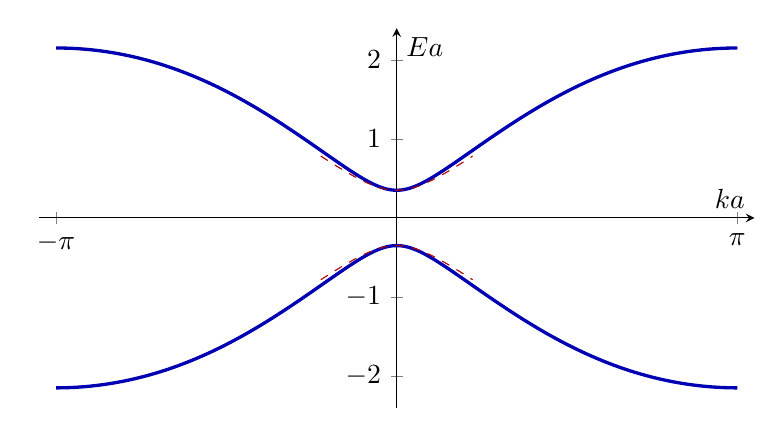
\begin{tikzpicture}
\begin{axis}[
  width=0.88\textwidth,
  height=6.4cm,
  domain=-3.1416:3.1416,
  samples=320,
  xmin=-3.3,xmax=3.3,
  ymin=-2.4,ymax=2.4,
  axis lines=middle,
  xlabel={\(ka\)},
  ylabel={\(Ea\)},
  xtick={-3.1416,0,3.1416},
  xticklabels={\(-\pi\),\(0\),\(\pi\)},
  ytick={-2,-1,0,1,2}
]
\addplot[very thick,blue!70!black] {sqrt((sin(deg(x)))^2 + (0.35 + 0.9*(1-cos(deg(x))))^2)};
\addplot[very thick,blue!70!black] {-sqrt((sin(deg(x)))^2 + (0.35 + 0.9*(1-cos(deg(x))))^2)};
\addplot[dashed,red!70!black,domain=-0.7:0.7] {sqrt(x^2 + 0.35^2)};
\addplot[dashed,red!70!black,domain=-0.7:0.7] {-sqrt(x^2 + 0.35^2)};
\end{axis}
\end{tikzpicture}
\caption{Efecto cualitativo del termino de Wilson en \(1D\). El modo ligero cerca de \(k=0\) sobrevive, mientras el doblador del borde adquiere una masa mucho mayor.}
\label{c26:fig:wilson}
\end{figure}

\section{Otras estrategias conceptuales}

Para el proyecto conviene registrar, aunque sea de forma resumida, las salidas mas importantes:

\begin{enumerate}[leftmargin=*]
  \item \textbf{Wilson:} elimina dobladores haciendolos pesados, a costa de romper quiralidad de forma explicita en la red;
  \item \textbf{staggered fermions:} redistribuyen componentes espinoriales entre sitios y reducen parcialmente el numero de especies;
  \item \textbf{domain-wall / overlap:} introducen una construccion mas sofisticada para preservar mejor la quiralidad efectiva;
  \item \textbf{aceptar pares de nodos:} en grafeno y en semimetales de Weyl, los duplicadores no son un defecto del modelo sino parte de la fenomenologia.
\end{enumerate}

La eleccion entre estas rutas depende del objetivo final:

\begin{enumerate}[leftmargin=*]
  \item si queremos modelar un material, el emparejamiento de nodos es aceptable y fisicamente correcto;
  \item si queremos una teoria fundamental quiral en red, el problema es mucho mas severo;
  \item si queremos un ansatz de espacio-tiempo discreto, debemos decidir con claridad cual de esos dos escenarios perseguimos.
\end{enumerate}

\section{Mapa de lectura dentro del programa}

Podemos resumir la logica de la escalera conceptual asi:

\begin{figure}[ht]
\centering
\begin{tikzpicture}[>=Latex,node distance=1.5cm]
  \node[draw,rounded corners,fill=blue!6,align=center,minimum width=3.1cm,minimum height=1.05cm] (ssh) {SSH\\Dirac \(1+1\)};
  \node[draw,rounded corners,fill=blue!6,align=center,minimum width=3.1cm,minimum height=1.05cm,right=of ssh] (graphene) {Grafeno\\Dirac \(2+1\)};
  \node[draw,rounded corners,fill=blue!6,align=center,minimum width=3.1cm,minimum height=1.05cm,right=of graphene] (weyl) {Weyl/Dirac \(3D\)};
  \node[draw,rounded corners,fill=orange!10,align=center,minimum width=3.9cm,minimum height=1.05cm,below=1.25cm of graphene] (nn) {Nielsen--Ninomiya\\y doblamiento};
  \node[draw,rounded corners,fill=green!8,align=center,minimum width=3.6cm,minimum height=1.05cm,below=1.25cm of nn] (future) {\(3+1\) discreto\\QW / QCA o Hamiltonianos};

  \draw[->,thick] (ssh) -- (graphene);
  \draw[->,thick] (graphene) -- (weyl);
  \draw[->,thick] (graphene) -- (nn);
  \draw[->,thick] (weyl) -- (nn);
  \draw[->,thick] (nn) -- (future);
\end{tikzpicture}
\caption{Ubicacion de este capitulo en el programa de investigacion. El doblamiento fermionico no es un detalle tecnico posterior: es el cuello de botella entre la intuicion de red y la ambicion de llegar a \(3+1\).}
\label{c26:fig:roadmap}
\end{figure}

\section{Resumen final}

El contenido esencial de este capitulo puede comprimirse en cuatro ideas:

\begin{enumerate}[leftmargin=*]
  \item una discretizacion local simple reemplaza el momento lineal por funciones periodicas en la zona de Brillouin;
  \item esa periodicidad genera ceros extra del operador de Dirac en red;
  \item en \(d\) dimensiones, la discretizacion ingenua produce \(2^d\) especies ligeras;
  \item la cancelacion global de quiralidad en la zona de Brillouin es la raiz geometrica del teorema de Nielsen--Ninomiya.
\end{enumerate}

Para el proyecto, esto significa que no basta con construir una red cuya teoria efectiva \enquote{se parezca} a Dirac. Hay que decidir que se hace con los dobladores y bajo que interpretacion fisica se los acepta, se los elimina o se los reubica.

Ese es precisamente el paso que prepara el salto serio hacia un modelo \(3+1\) con pretensiones mas fundamentales.
